\documentclass[a4paper]{article}
\usepackage[T1]{fontenc}
\usepackage[russian]{babel}
\usepackage[pdftex]{graphicx}
\usepackage[ruled,vlined]{algorithm2e}
\usepackage[utf8]{inputenc}
\usepackage{xcolor}
\usepackage{hyperref}
\usepackage{amsmath}
\usepackage{geometry}
\usepackage{float}
\usepackage{caption}
\usepackage{subcaption}
\DeclareGraphicsExtensions{.pdf,.png,.jpg}

\begin{document}

    \begin{titlepage}
        \Large
        \begin{center}
            Санкт-Петербургский \ Политехнический университет Петра Великого\\
            \vspace{10em}Отчет по лабораторной работе №1\\
            \vspace{2em}
            \textbf{Изучение характеристик распределений}
        \end{center}
        \vspace{6em}
        \hfill\parbox{10cm}{
            \hspace*{2cm}\hspace*{-4cm}Студент:\hfill Швачко Никита Андреевич\\
            \hspace*{2cm}\hspace*{-4cm}Преподаватель:\hfill Баженов Александр Николаевич\\
            \hspace*{2cm}\hspace*{-4cm}Группа:\hfill 5030102/20202
        }
        \vspace{\fill}
        \begin{center}
            Санкт-Петербург \ 2025
        \end{center}
    \end{titlepage}


    \section{Формулировка задания и его формализация}\label{sec:----2}
    Для 4 распределений:
    \\- Нормальное распределение $N(x, 0,1)$
    \\- Распределение Коши $C(x, 0,1)$
    \\- Распределение Пуассона $P(k, 10)$
    \\- Равномерное распределение $U(x,-\sqrt{3}, \sqrt{3})$
    \\1. Сгенерировать выборки размером 10,50 и 1000 элементов. Построить на одном рисунке гистограмму и график плотности распределения.
    \\2. Сгенерировать выборки размером 10,100 и 1000 элементов. Для каждой выборки вычислить следующие статистические характеристики положения данных: $\bar{x}, \operatorname{med} x, z_Q$. Повторить такие вычисления 1000 раз для каждой выборки и найти среднее характеристик положения и их квадратов:

    $$
    E(z)=\bar{z}
    $$


    \\  Вычислить оценку дисперсии по формуле:

    $$
    D(z)=\overline{z^2}-\bar{z}^2
    $$


    Представить полученные данные в виде таблиц.
    \\ Пояснение

    $$
    z_Q=\frac{z_{1 / 4}+z_{3 / 4}}{2}
    $$


    \section{Гистограммы и графики плотности распределений}\label{sec:----}
    \begin{figure}[H]
        \centering
        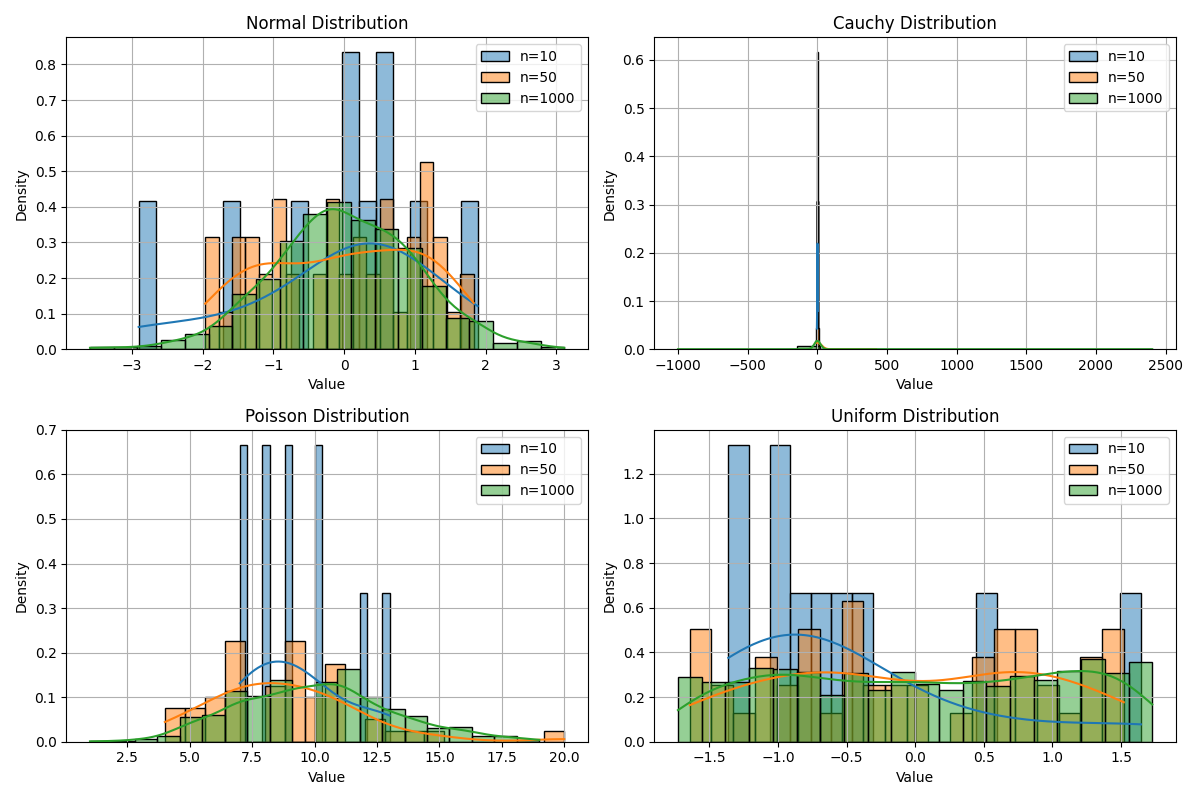
\includegraphics[width=0.8\textwidth]{../histograms} % Вставить график
        \caption{Гистограммы и плотности распределений для выборок разного размера}\label{fig:figure}
    \end{figure}


    \section{Результаты вычислений статистических характеристик}\label{sec:---}
    \begin{table}[H]
        \centering
        \caption{Средние значения характеристик положения и их дисперсии}
        \begin{tabular}{|c|c|c|c|c|}
            \hline
            Размер выборки & Статистика     & $E(z)$    & $D(z)$   \\
            \hline
            10             & mean           & -0.008095 & 0.102135 \\
            10             & median         & -0.004625 & 0.135981 \\
            10             & quartile\_mean & -0.010810 & 0.117080 \\
            100            & mean           & 0.000288  & 0.010116 \\
            100            & median         & 0.000817  & 0.015189 \\
            100            & quartile\_mean & 0.003888  & 0.012624 \\
            1000           & mean           & 0.000635  & 0.001005 \\
            1000           & median         & 0.001211  & 0.001609 \\
            1000           & quartile\_mean & 0.000023  & 0.001208 \\
            \hline
        \end{tabular}
        \label{tab:table}
    \end{table}


    \section{Выводы}\label{sec:}
    \begin{itemize}
        \item При увеличении размера выборки характеристики положения стабилизируются.
        \item Среднее значение $\bar{x}$ для распределения Коши не является надежным из-за сильных выбросов.
        \item Медиана и квартильный средний $z_Q$ показывают меньшую изменчивость в выборках с выбросами.
        \item Пуассоновское распределение при больших $n$ приближается к нормальному.
        \item Равномерное распределение демонстрирует низкую изменчивость статистик.
    \end{itemize}


\end{document}
